\chapter{Implementation}
\label{chp:implementation}
\section{Components}
\subsection{Web3 Framework}
Web3.js \cite{ethereum_foundation_web3.js_nodate} is a JavaScript interface for Ethereum which conforms to the Generic \ac{JSON} \ac{RPC} Specification \cite{ethereum_foundation_ethereum_nodate} used by other Ethereum clients. It can send transactions, call functions in smart contracts and compile and deploy Solidity smart contract code.

Web3 was chosen as the interface for interacting with the Ethereum smart contracts, as it is a platform-independent framework that operates client-side and within the browser. Web3 can use a local Ethereum node for testing purposes, or it can be pointed at a remote node connected to the Ethereum \textit{Test Net} or \textit{Main Net}. Infura \cite{noauthor_infura_nodate} is a service that offers public Ethereum nodes that serves blockchain \ac{RPC} requests for applications.

\subsection{Transaction Signing}
Transaction signing is not offered by Web3, but it can be offloaded to the connected Ethereum node if the keys of the requested account are stored on the node. To enable local transaction signing in the client, packages like ethereumjs-tx \cite{noauthor_ethereumjs-tx_nodate} and ethereumjs-util \cite{noauthor_ethereumjs-util_nodate} can be added to the project. These packages use private keys stored locally to sign transaction requests, and they subsequently send raw transactions to the Ethereum node.

Metamask \cite{noauthor_metamask_nodate} is another project for Ethereum account management that runs as a browser extension. It stores the public and private keys for Ethereum wallets in the browser local storage and supports client-side transaction signing.

\subsection{TestRPC}
TestRPC \cite{noauthor_testrpc_nodate} can be used for rapid testing of Ethereum smart contracts and applications. It simulates a full Ethereum node and local blockchain network. It can generate a number of addresses with initial balances and store their keys on the node. It also mines blocks of transactions instantly to facilitate faster development.

The implementation of this project uses TestRPC, but it could be easily changed to point to an Ethereum node connected to the live blockchain. TestRPC was convenient as it gave generated wallets initial account balances, which removed the need for mining Ether to fund contract deployments and transactions.

\subsection{IPFS}
A local \ac{IPFS} node was set up to store user identity data during development. This could also be easily pointed to a public \ac{IPFS} node such as one hosted by the organisation themselves.

Data on \ac{IPFS} follows a standard format for storing attributes and signatures. An example is shown below.

\begin{spacing}{1}
  \inputminted{json}{./code/IPFS.json.txt}
\end{spacing}
Example snippet hash: \textit{QmUHxAMb53UeAY6srn9xEBUthcBVT5sVrRRJrbwwkqxy3Z}.

\section{Interface}
\subsection{Main Screen}
The primary interface of the implementation is shown below in Figure \ref{fig:home-screen}. It displays the user's \ac{UUID}, their name attribute, Ethereum wallet balance, device public key, recovery contract address and \ac{IPFS} content hash.

\begin{figure}[ht]
\centering
     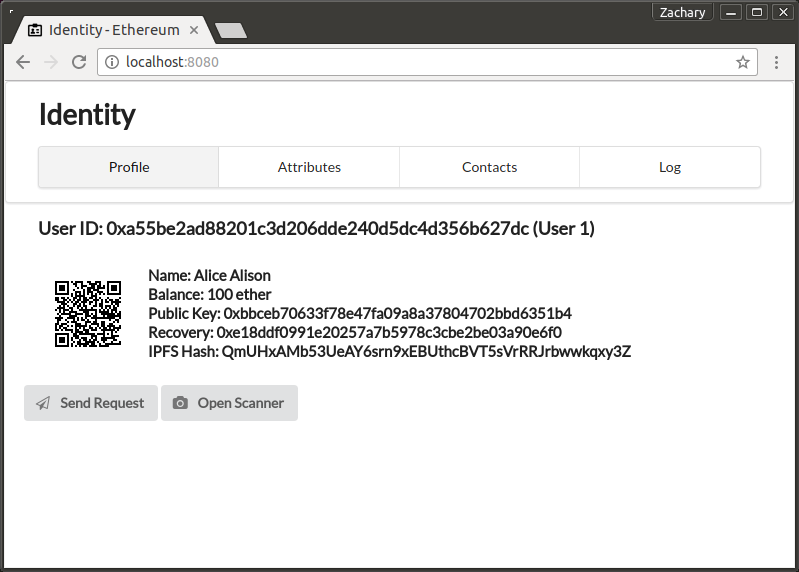
\includegraphics[width=1.0\textwidth]{./images/HomeScreen.png}
      \caption{Home Screen: Initial view of a user's identity on the platform.}
       \label{fig:home-screen}
\end{figure}

The \ac{UUID}, which is also the address of the user's identity contract, is stored in the local storage of the browser. This is then used to fetch the rest of the user's data.

\subsection{Data Transfer}
\label{sec:data-transfer}
QR codes were chosen as the transport protocol to transfer information between parties in the system. This can be replaced with any other peer-to-peer messaging protocol like Bluetooth or Wi-Fi Direct. Ethereum has plans to release a dedicated protocol known as Whisper  \cite{ethereum_foundation_whisper_nodate} which could also be used in the future.

An example of the QR code used to transmit a signature request is shown in Figure \ref{fig:signature-request} below. This shows the accompanying \ac{JSON} value that contains the user's \ac{UUID}, the name of the attribute to be signed, and the value. This can be scanned by a third party, approved, and then the attributes signed and returned.

\begin{figure}[ht]
\centering
     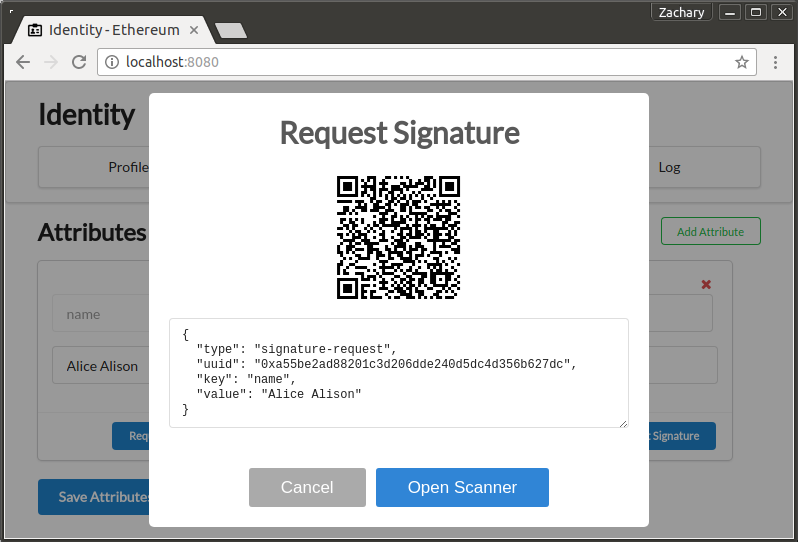
\includegraphics[width=1.0\textwidth]{./images/SignatureRequest.png}
      \caption{Signature Request: An example using a QR code to request a signature.}
       \label{fig:signature-request}
\end{figure}

A table of the possible message types is also shown in Table \ref{tab:message-types} below. These are read by the JavaScript implementation and present different dialog boxes to the user.

\begin{table}[H]
	\centering
    \begin{tabular}{|p{4cm}|p{8cm}|}
       \hline \textbf{Message Type} & \textbf{Attributes} \\
       \hline contact-card & uuid \\
       \hline signature-request & uuid, key, value \\
       \hline attribute-request & attributes, uuid \\
       \hline recovery-request & uuid, new-key \\
       \hline signature-result & key, value, signer, signature \\
       \hline disclosure-result & uuid, attributes, signature \\
       \hline
    \end{tabular}
    \caption{Message types and values for passing data between users.}
    \label{tab:message-types}   
\end{table}

\section{Additional Features}
\subsection{Deterministic Wallet Seed}
Another recovery mechanism that could be added to the system is a recovery mnemonic, a human readable seed that is used to generate the public and private key pair.

A \ac{BIP} known as \ac{BIP}39 \cite{noauthor_bip-0039_nodate} was released in 2013 to help users make a backup of their digital currency wallets. It builds upon the advancements of deterministic wallet generation from a given seed brought about by \ac{BIP}32 \cite{noauthor_bip-0032_nodate}.

A twelve or sixteen-word seed is generated from a list of 2048 English words. This mnemonic is then hashed and converted into a seed value for the key generation function. \textit{Hierarchical Deterministic} wallets allow an infinite amount of addresses to be generated from a given seed, using an index value.

Human readable seeds can thus be given to the user to write down on paper, and they allow multi-currency addresses to be recovered. This should act as the primary backup feature for the user's identity, as it is simpler than coordinating with multiple backup contacts.


\subsection{User Attribute Privacy}
\label{sec:user-attribute-privacy}
User attributes are stored unencrypted on \ac{IPFS} and linked directly to the user's \ac{UUID}. This means that whenever the \ac{UUID} is shared, the receiving party can view all the public attributes and signatures relating to that user. Other existing implementations such as uPort as seen in Section \ref{sec:uport} allow the use of privately stored attributes that are not on the blockchain, but recovery of these is not possible in cases of device compromise.

A proposed solution is to have a second "encryption key" in addition to the device signing key owned by the user. This encryption key would be used to encrypt all user data before publishing it to the public blockchain. Disclosure of attributes is done by downloading this encrypted data, and then decrypting it before encrypting with the receivers public key for transport.

As private data cannot be stored in Ethereum smart contracts, the encryption key is not recoverable using the blockchain. The function of storing encrypted data in smart contracts that they can act on is known as secure multi-party computation \cite{andrychowicz_secure_2014} and remains largely unsolved for blockchain technology. Some facility is therefore required to enable recovery contacts to restore a user's encryption key, to avoid them losing their stored private data.

\textit{Threshold cryptography} \cite{desmedt_threshold_1994} is proposed to solve this, which allows a piece of data to be split such that M of N pieces need to be combined to restore it. It allows secure sharing of a secret value such that no less than the specified number of peers can come together to reveal the data.

The private encryption key of the user could, therefore, be split using the threshold cryptography algorithm, and encrypted with the public keys of the user's recovery contacts. In the event of key loss or compromise, the user can request the decrypted values from M of N contacts and then run the data back through the algorithm to restore their private key.